\chapter{The Envoy Prototype}

\section{Scope and design coverage}

\section{Mapping to the 9p protocol}
\section{Synchronization}

\section{Storage service}

Storage instances are stateless and unaware of higher-level semantics with two exceptions:

\begin{enumerate}
\item Each storage instance can respond to a reservation request, which returns a range of object IDs that have not been used or allocated on that particular instance.
\item The \emph{clone} operation, which copies an object from one given ID to another, will expect objects whose attributes indicate that they are directories to follow a particular format (described in \prettyref{sec:directory-format}) and will set the copy-on-write flags within each block as it copies the object.
\end{enumerate}

Neither of these functions is essential for implementation in the storage layer. The first could easily be performed by a different service (such as an elected instance of the envoy service) and the second is merely a performance optimization. Both are convenient to implement in the storage layer, however, so they are there in the prototype.

\section{Envoy service}

Having examined the high-level architecture of the Envoy file system, I next turn to a more detailed discussion of how specific operations are served. This includes basic file operations and navigation between envoy instances, the copy-on-write mechanism behind the fork and snapshot operations, coordination of state during territory boundary realignment, security considerations, and the procedure for deleting file system images.

For operations that require the synchronous cooperation of multiple envoy instances, dependency cycles and deadlock become a concern. To minimize these issues, Envoy is designed with a top-down locking protocol where synchronous operations only directly involve immediate neighbors in the tree of territories, and owners of territories closer to the root always initiate and coordinate transactions with those lower in the tree. While operations with wide-ranging impact may require communicating with every node in the cluster, they never require a cycle in the connectivity graph and are not prone to distributed deadlock.

\subsection{Freezing and thawing}

Synchronization at the object level is governed by an important invariant: an object in the system may be referred to by exactly one name in the hierarchical namespace, or it must be read-only. The storage layer makes no attempt to detect or enforce the read-only case, so it is left to the envoy layer to ensure that this invariant is preserved. To make this straightforward, objects can transition from being writable to read-only, but they can never go back. Note that this refers only to objects in the storage layer, not to the access control of file system objects.

The same invariant makes cache management simple: the envoy that owns a given territory can cache it without any invalidation concerns, and read-only objects can be safely cached at any number of envoy nodes without fear of interference. Objects in the cache become invalid only when a territory boundary changes. Objects that are part of ceded territory are not explicitly flushed from the cache; keeping them active helps in two cases: a read-only object may still be referenced by another name in a local territory, and the cache entry (in-memory or on-disk) may still be useful if a file backed by that object is later returned to local control. In the latter case the object must be verified to match the version in the storage layer, but this can be done with a lightweight metadata comparison.

The single mutable/multiple immutable dichotomy in the storage layer is tracked in the envoy layer through the copy-on-write flag in directory entries. The immutable property is not directly assigned to objects, but instead is imbued by the link from directory to file object. Furthermore, when the immutable object is itself a directory, the property is applied recursively to all of its children, overriding the individual copy-on-write flag in the link to each child. To be regarded as mutable, an object must be reachable by a path from the root of the global namespace to the directory entry linking to the object without traversing any copy-on-write flags that are set.

One immediate consequence of this is that taking a read-only snapshot of a directory and its descendents requires only setting the copy-on-write flag in the link to it, an operation known as \emph{freezing}. Once a directory or file is frozen, the storage layer objects that back the branch rooted at that point are considered immutable. To simplify bookkeeping, this operation is only performed from the root of client images when a snapshot operation is requested. The benefits gained from this restriction and an exception to it are discussed in \prettyref{sec:hard-links}.

The complementary operation is called \emph{thawing}. While the freeze operation works at the root of a subtree and affects it in its entirety, thawing aims to leave as small a footprint as possible; it is always performed with the goal of modifying a particular file. To thaw a file, the owning envoy starts walking up the line of its ancestors until it finds one that is already thawed. As the root of the namespace cannot be frozen (one can consider it as having a single, implicit link from the envoy service itself, but there is no mechanism provided to set the copy-on-write flag on this implicit link), this search is guaranteed to succeed. From there the envoy walks back to the target file, \emph{cloning} intermediate directories as it goes. In addition to making a copy of the directory as its name implies, cloning sets the copy-on-write flag of every directory entry in the copy, effectively transferring the copy-on-write property from the single link leading into the directory to all the links leading out of the directory. The implicit property that each child inherited becomes explicit after being passed down a generation. After thawing each directory for mutability, the parent is updated to reflect both the new object ID and the cleared flag. Eventually the intended target itself (be it file or directory) is cloned, its immediate parent link updated, and the file is fully thawed.

Thawing resembles the procedure for modifying a value in a tree in a functional language. In addition to changing the value itself, the path from that item to the root of the tree must be copied if the item is to be reachable from the root. In the thawing operation, it is only the root of the immutable subtree in which the item resides that must be copied. While the analagous procedure in a functional language copies everything exactly except for the path being changed, the thaw operation must clear the copy-on-write flag as it goes, and thus must push it down from parent link to sibling links at each level in order to preserve the immutable status of the unaffected branches.

\subsection{Read operations}

Most basic file and directory operations have a straightforward implementation. The need to cross territory boundaries makes some more complex, however, as they must coordinate with remote envoys to complete.

\subsubsection{Reading files and attributes}

The most straightforward operations are \texttt{read} and \texttt{stat}, which read the data and metadata of files, respectively. These requests can be filled using the data paths described in \prettyref{sec:data-paths-read}. The only complication involved is handling the \texttt{atime} attributed, which tracks the last time the data from a file was accessed by a \texttt{read} or \texttt{write} operation. Read operations always proceed through a single envoy, so this attribute can be tracked accurately: the envoy can send a message with the timestamp (to ensure that it is consistently applied to all replicas, even if all clocks are not in sync or network latencies between the different storage servers vary) to all replicas in the storage layer which can then update the attribute.

The intended meaning of the \texttt{atime} attribute becomes obscured when applied to frozen files, however. Since attributes are part of the object, akin to \texttt{inodes} in traditional Unix file systems, changing the attribute will affect all files that are backed by that same object. Those instances may be in read-only snapshots of the same file system image, or in common files available in an unrelated file system image. In the former case, the read-only property of the snapshot is broken, and in the latter case the isolation of the two images is compromized. Updating the \texttt{atime} attribute would give an unrelated client using the same prepackaged file system image the ability to losely track file accesses, which could represent a security risk.

Accurately tracking the \texttt{atime} attribute is problematic with frozen files, and if it is only updated on some files (which may change over time as successive snapshots are taken), it is too unreliable to be useful. It also generates network and disk traffic for every read, even those that can be satisfied from the cache. For these reason, the \texttt{atime} attribute is present in Envoy for compatibility, but it effectively mirrors the modified time attribute.

\subsubsection{Reading from directories}\label{sec:walk-cache}

Reading from directories introduces two complications. The first---that successive \texttt{readdir} requests require state that must be transmitted from the client each time or transferred to another envoy when territories are realigned---is just an implementation issue. The second---that a directory may span multiple territories---requires the cooperation of all affected envoys. The list of contents for a single directory is considered an atomic unit when drawing territory boundaries, but the files and directories named may be remote. If the client-server protocol used to export the file system to a service only requests names, then the implementation footprint resembles that of file reads. If the response includes attributes as well---as with 9p---additional requests must be forwarded to the respective envoys for all files that are across a boundary in order to ensure consistent results. These requests are sent directly by the owning envoy, so if the client is remote, \texttt{readdir} may require the cooperation of three or more envoys to complete a single request. When gathering file attributes, the envoy that owns the directory sends requests directly to the file owners, resulting in a star topology with the directory owner as the central node. An additional link from the client's envoy is necessary if the directory is remotely owned.

Multi-step directory navigation can also create a star pattern of requests, but they always center around the client's local envoy. Navigating down a series of directories---an operation called \texttt{walk} in 9p---may involve crossing a territory boundary at each step in the extreme case. Because an envoy confines itself to knowledge of its local territories and their immediate boundaries, it cannot always predict the endpoint envoy for a navigation. Even if it could, intermediate steps must always be taken to allow permission checking at each level. When a remote territory must be consulted, the client's envoy forwards all remaining steps in the \texttt{walk} to the remote owner, which proceeds as far as it can with the navigation. It may return one of three results: if the result is successfully completed, the two envoys store any state necessary to handle future requests; if the result is a failure, an appropriate error code is returned; if the navigation reaches another territory boundary, the partial result comes back along with a pointer to the envoy that must be consulted to continue the navigation. The client's envoy then repeats the procedure with the remaining navigation steps.

Because these operations are all asynchronous, and because the navigated directories may be owned by remote envoys that are not even neighbors to the client's envoy, \texttt{walk} may encounter transient failures. Between the time that one remote envoy returns instructions for forwarding the remainder of a request, the target territory may migrate to a new owner and the request will fail. Because the envoy that sent the forwarding instructions was an immediate neighbor of the target, its information must have been correct at the time, and careful coordination can ensure that by the time the target bounces the request back with a failure notice, the referrer knows of the change to its immediate neighborhood. The solution is simply to restart the request from the beginning, which will also correct the client's envoy for the cases of a directory being deleted or renamed.

Generally, having territory boundaries closely aligned with demand benefits everyone, but if multi-step directory navigations are frequent, their performance will be hurt by frequent boundary crossing. Caching \texttt{walk} results can be done safely with a few precautions. First note that a navigation that succeeds one time and fails another implies one of three things: one of the steps was deleted or renamed, permissions changed somewhere, or a different user requested the navigation. The prototype caches \texttt{walk} results keyed by the path traversed and the user that requested it. With the assumption that directory renames and permission changes are uncommon (particularly across boundaries determined by locality of reference---I expect these changes to be most common in a region being actively modified by a single player, not in higher-level directories whose descendents are in active use by different clients), envoys broadcast notification of such changes down the hierarchy when they occur, invalidating cached navigation results. The notification of permission changes is treated as a special case of directory renaming for cache invalidation purposes, as discussed in \prettyref{sec:rename-operation}.

Attributes at the endpoint of the navigation are always confirmed directly with the owner, as are all of the final steps that occurred on territory owned by that same envoy. With a hot cache, multi-step directory navigations are satisfied from the cache of the client's envoy and a single step to the envoy hosting the target of the navigation.

\subsection{Write operations}

\subsubsection{Writing data and attributes}

Like the corresponding read operations, writes to files and changes to file metadata are largely a matter of directing the request to the appropriate envoy. The first change to a file since a snapshot or fork will first require the file to be thawed, but subsequent changes can be made directly to the local cache entries and propogated to all replicas in the storage layer. As discussed in \prettyref{sec:data-paths-write}, changes are considered complete when they have been received by all storage servers, but not necessarily commited to stable storage.

To ensure consistent time stamps, the modification time is determined by the envoy that owns the file and transmitted to the storage layer along with the data being written. While the clocks of machines within a cluster can be synchronized within reasonable bounds, network latencies and variations in storage server load levels would make it difficult to rely on strict synchronization for consistent timestamps. The envoy is a natural location for deciding on the canonical time for its territories.

Thawing a file requires walking back in the file tree until an already-thawed directory is found. To bound the complexity of this procedure and to avoid deadlocks, the root of every local territory is always thawed unless it is part of a read-only snapshot image. While thawing may require cloning multiple levels of the directory hierarchy, this confines the direct impact to a single envoy. It also preserves the top-down rule for synchronous inter-envoy operations by preventing an envoy from demanding a bilateral change from its parent in the tree of territory ownership.

\subsubsection{Deleting files}

The \texttt{inode}-like disconnect between directories and the files they name means that one envoy may own a territory consisting of a single file, while another envoy owns the directory containing that file. Most operations involve either the file itself or the directory, but not both, so it is obvious which envoy should serve the request. Removing a file or directory is a case where the possibility of divided ownership complicates the implementation.

Deleting a file affects both envoys in this case, but the operation needs to appear atomic to clients. The normal rule in Envoy is that the parent should drive bilateral operations, meaning in this case that the owner of the directory should coordinate the removal with the owner of the file. This is a mismatch with 9p, where removal is an operation initiated on a file, not on the directory that contains it.

A higher-level consideration ultimately drives the design of the delete operation, however. Removal can only succeed on files or empty directories, so an envoy that owns the target of a successful delete will have nothing left to own afterward. Instead of trying to atomically coordinate a multi-step the operation between two envoys, the parent instead revokes ownership of the child from its envoy and reclaims it before proceeding.

Since 9p initiates removal with the file to be deleted and not its containing directory, this requires a minor slight-of-hand to maintain the top-down coordination rule. A \texttt{nominate} request is sent from the file's envoy to the that of the parent directory, requesting that it reclaim the removal target. Since \texttt{nominate} operations are implemented strictly in terms of names (not 9p file handles) this request cannot trigger a deadlock, and the remove transaction running on the child envoy effectively becomes a passive observer while control of the territory is transferred. After the transfer is complete, the envoy aborts the transaction and starts it over. Since the file is no longer local, the envoy will either forward the request (if it happens to be the client's local envoy) or reject it, forcing the client's envoy to redirect it to the new owner. \texttt{nominate} requests do not return until all state has been transferred, so the restarted transaction can proceed immediately.

Deletes happen in four basic steps. The first checks that the file is a suitable candidate for deletion, namely that it is a file or an empty directory. The second verifies that the client has permission to remove it from the parent directory, and the third actually removes it. In the case where the territory ownership must change, the envoy owning the file can complete the first step, but it does not know if the second step will succeed and blindly proceeds to initiate the transfer of control. This could cause unnecesary activity if the permission check fails, but in practice the Linux driver used in the prototype does an explicit check before making the delete request, so the possibility of failure is remote: it would indicate an uncommon race condition and does not compromise the correctness of the operation even then.

The fourth step in deleting a file is to actually delete the object that backs it and reclaim the storage space. This is simple enough to do, but deciding when to do it is slightly more complicated. An object can only be deleted when no more names link to it, and to support Unix semantics it should also be preserved until all clients accessing it have closed the file. The former case is easy to detect: if the link to the file was marked as copy-on-write, it shares a link with at least one snapshot and should not be removed. Otherwise, it was created or cloned in the current image since the most recent snapshot and can be safely removed.

To support familiar Unix semantics, the envoy instance strips waits until all file handles are closed before deleting the file. 9p is stateful, so this is straightforward, but it does create a few corner cases that must be dealt with. A new file with the same name could be created, so the envoy cannot continue to track the object by its former name. Without a name the file does not belong to any territory, so it becomes an orphan. Opening a file and deleting it is often done to provide a temporary scratch file that will delete itself if the process dies, but it may still be long-lived. The envoy must still be prepared to thaw it if it was frozen at delete time, migrate it to another envoy in response to demand or to the owning envoy shutting down, and delete the storage layer object even in the event of a failure. The prototype does not address all of these issues, but it does support arbitrary use of the file until the last file handle is closed, at which point the object is deleted from the storage layer if appropriate.

\subsubsection{Renaming files}\label{sec:rename-operation}

Renaming a file exposes the same coordination issues as deleting a file. In 9p a rename request is part of a \texttt{wstat} request, which treats the file name as a property of the file object rather than of the directory that contains it. With rename the issue is even worse than with delete, because up to three objects and three envoys may be involved: one owning the directory, one owning the file to be renamed, and the third owning an old file with the target name that will be implicitly deleted when the rename completes. To further complicate the issue, Unix programs assume that rename-with-delete will complete atomically. Note that the original 9p protocol does not support this (it calls for a failure if the target name is already in use) but the Linux implementation does support this arrangement, and many clients demand it.

As with delete, the prototype simplifies the problem by consolidating ownership of all participanting objects onto a single envoy before making any changes. Unlike the delete case, the renamed file exists afterward and may be a non-empty directory. If it was owned by a different envoy before, that envoy probably drives most of the traffic to it and annexing it into the parent territory may be a poor move for matching ownership with usage. One solution would be to transfer control back to the original owner after the rename completes. It would have to revalidate some cache entries, but they would still be mostly unchanged, and even the in-memory cache would still be usable after a single metadata check on each file. A second possibility would be to engineer a distributed version of rename for these cases, driven by the parent (as with all synchronous operations) and handling transient failures appropriately. A third approach (the simplest and the one taken by the prototype) is to assume that such renames are rare and do nothing. Correct behavior is still maintained, and eventually traffic patterns will force the owner to cede the territory once again if appropriate.

Renames of directories present another difficulty that cannot be safely ignored. Territory boundaries are all managed using directory and file names, so renaming a directory that is ancestor to other territories throws management state out of sync. On the assumption that renaming high-level directories is relatively rare, the prototype handles them by propogating rename events from parent territory to child and from owner envoy to client envoy when they happen, rather than trying to assign immutable aliases for directories or some other similar scheme. Minor overhead in the rare case is usually preferable to complexity in every case.

In addition to updating territory and file handle names, these tree-traversing rename messages flush the walk cache described in \prettyref{sec:walk-cache}.  While a more fine-grained invalidation could be implemented, in practice an occasional flush has very little affect on performance, and it offers a mechanism for solving another problem. As a special case, this message can be used to rename a directory to the same name, forcing a recursive flush of the walk cache but not changing anything else. This is useful when directory ownership or attributes change, and walk operation results that have been cached may no longer be valid. Since this is expected to be rare, it forces a broadcast down the name hierarchy when it happens, rather than forcing checks whenever the walk cache is consulted.

\subsubsection{Hard links}\label{sec:hard-links}

Unix file systems allow multiple names to refer to the same file. While symbolic links merely contain the name of their target, hard links allow multiple links from directories to resolve to the same \texttt{inode}. File operations are coordinated internally with reference to the \texttt{inode}, not the file path, so handling concurrent access is no different than if the clients all opened the same file through the same name. Because \texttt{inode} numbers are only meaningful in the context of a file system, hard links are not permitted across file system mount points. This mechanism is widely used both for aliasing, where two names are given to the same file, and as a way of moving a file without copying it, where the original name is unlinked after the alias has been created. 9p does not support hard links, but the Linux extensions to it do.

While Envoy's structure of names and object IDs resembles the Unix system of file paths and \texttt{inodes}, it does not behave quite the same way. Access coordination in Envoy is done with reference to file names, not storage layer object IDs. When the latter are shared, the objects are assumed to be read-only and can be cached freely on different nodes with no attempt to synchronize access. Different references to the same object ID, even within the same file system image, may be split into different territories and owned by different envoy instances.

For this reason, Envoy offers only partial support for hard links; a file must be frozen before additional names can be linked to it. If futures changes are made to the file through any of its references, the changed versions will be thawed independently and will diverge.

The implementation of the hard link operation is also unique in that the client's envoy intercepts the request before passing it on to the owning envoy if the link is being created in a foreign territory. The Linux extensions to 9p implement hard links by walking to the target of the link, then creating the new link as a file with a special extended attribute containing the file handle of the referent. The file handle state is only available to the client's envoy, so it uses the handle to freeze the target file (if necessary) and rewrites the request to include the object ID instead of the file handle. The envoy (remote or local) can then link the new name to the object.

\subsection{Modifying territory ownership}

Misaligned boundaries do not prevent correct behavior, nor do they introduce a heavy performance penalty. The algorithms to trigger changes are designed to promote good long-term layout choices based on steady-state traffic patterns. Cache effects penalize excessive changes, while the low network latency in a cluster environment reduces the cost of relying on a remote envoy even when local ownership would be preferable. In centralized server systems, all file access is routed across a high-speed LAN to a server with many clients. In Envoy, this pattern is also quite servicable, even when it is not ideal, and Envoy is designed to favor gradual, long-term changes over a quick response in short-term traffic patterns.

Realigning territories requires careful coordination between multiple envoys. In addition to agreeing on new boundaries, state related to active file handles has to be migrated and updated. This includes both the territory owner's state and that of the envoys representing clients, which need to be directed to the new owner. Inflight operations---those that have been initiated by a client but not completed---must also continue and succeed despite concurrent territory changes.

The prototype is designed to make territory migration simple and clear. Performance for infrequent operations has little bearing on the overall performance of the system \cite{amdahl}, and I consider simplicity and an increased chance of correct behavior to be more important in a complex operation of a distributed system (especially a prototype) than optimal performance.

Like other operations involving multiple envoy instances, territory migration is driven by the owner of the parent territory, as illustrated in \prettyref{fig:grant-topdown}. If an envoy wants to merge a territory with its parent, or transfer it to another specific envoy, it sends a \texttt{nominate} request to the parent, giving the root path of the territory and the envoy to which it should be transferred. If a territory owner wants to cede part of a territory to another envoy or annex a neighbor that is a child of a local territory, it begins the process unilateraly. In practice, annexing is only done in response to a nomination from the child, but the process is always driven in a strict top-down fashion.

\begin{figure}[tp]
\centering
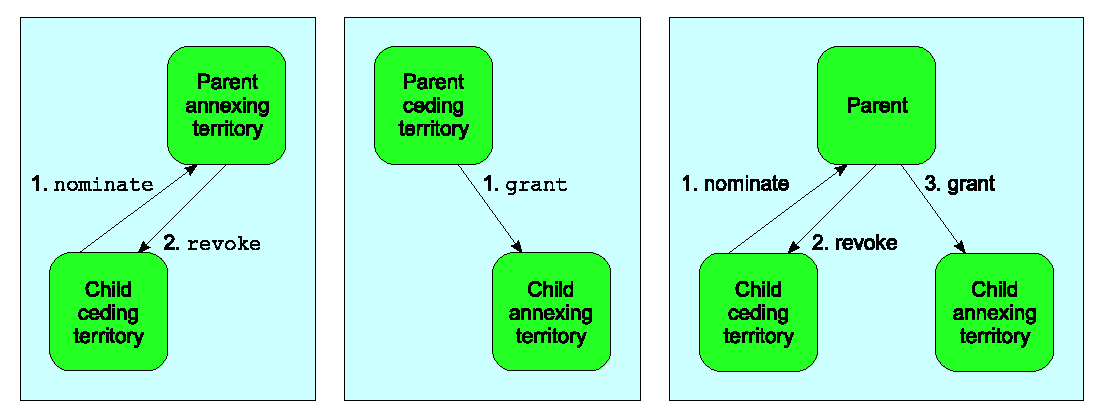
\includegraphics[width=100mm]{figures/grant-topdown}
\caption{Territory migrations are always driven by the parent in the namespace tree, which can annex a neighboring territory, cede territory to another envoy, or coordinates the transfer of a territory from one neighbor to another. For a child to initiate a transfer, it must send a \texttt{nominate} request to the parent, which then carries out the transfer.}
\label{fig:grant-topdown}
\end{figure}

\subsubsection{Transferring state}

Transfers occur

\subsubsection{Inflight operations}


\section{Caching}

\section{Summary}